\subsection{Estimate Classification Qualities without 
Testing Labels} 

In this section, we evaluate Algorithm \ref{alg:prediction} 
with four representative prediction models, namely, 
logistic regression, linear SVM, k-nearest neighbor 
and decision tree. 

We will first present a case study on the Spam Email data 
set, and then present extensive results on other data sets. 

{\noindent \bf A Case Study on Spam Email Data Set} 

We examined logistic regression on the Spam Email 
data set. The regularization coefficient of logistic 
regression was set to 10 based on 
our grid search results in Figure \ref{exp1:modelselection}. 

\begin{figure}[h]
\centering
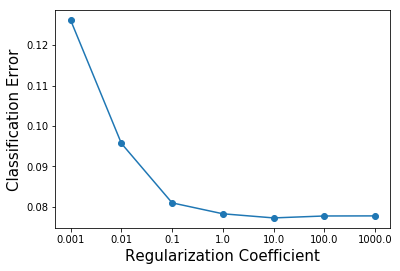
\includegraphics[width=4.5cm,height=3.25cm]{exp1_modelselection.png}
\vspace{-10pt}
\caption{Testing Error versus Regularization Coefficient}
\label{exp1:modelselection}
\end{figure}

First, we evaluated classification error. 
Recall $er(f; Q)$ is the testing error. 
Let $er(f; S)$ be the training error, and 
$\tilde{er}(f; S)$ be the reversed testing error. 
The estimation quality of $er(f; S)$ on $er(f; Q)$ 
is measured by 
\begin{equation}
\Delta_{tr} = | er(f; Q) - er(f; S)  |,  
\end{equation}
and the estimation equality of $\tilde{er}(f; S)$ 
on $er(f; Q)$ is 
\begin{equation}
\Delta_{retr} = | er(f; Q) - \tilde{er}(f; S) |.  
\end{equation}
Results are shown in Table \ref{exp1:classificationerror}. 
We see $\tilde{er}(f; S)$ is closer to $er(f; Q)$ 
than $er(f; S)$, which is a first empirical evidence 
that reversed testing quality is a more accurate estimate 
of testing quality than traditional training 
quality\footnote{More 
results of this experiment can be found in 
Table \ref{tab1:accf1}.}. 

\begin{table}[h]
\renewcommand{\arraystretch}{1.5} 
\caption{Classification Errors on Spam Email Data Set}
\centering
\begin{tabular}{l|ccccc} \hline 
\bf Metric & \bf $er(f; Q)$ & \bf $er(f; S)$ & \bf 
$\tilde{er}(f; S)$ & \bf $\Delta_{tr}$ & \bf 
$\Delta_{retr}$ \\ \hline 
\bf Value & .0686 & .0773 & .0733 & .0087 & .0040 \\ \hline 
\end{tabular}
\label{exp1:classificationerror}
\end{table}

Next, we evaluated the impact of sample size on 
estimation. We varied the fraction of training 
instances from 10\% to 90\% (with the remaining 
instances used for testing), and obtained results 
in Figure \ref{exp1:samplesize}. 
Wee see $\tilde{er}(f; S)$ remains a more accurate 
estimate of $er(f; Q)$ in most cases, except when 
testing sample is very small (less than 20\% of the 
data set). The latter suggests reversed testing 
quality is more effective when one has sufficient 
testing sample. 

\begin{figure}[h]
\centering
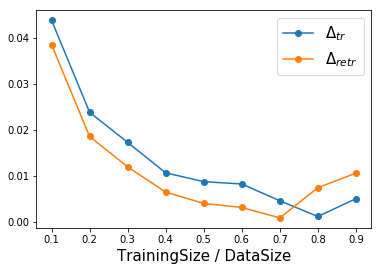
\includegraphics[width=5cm,height=3.5cm]{exp1_samplesize.png}
\vspace{-10pt}
\caption{Performance over Different Training Sample Size}
\label{exp1:samplesize}
\end{figure}

So far, we have been retraining $f$ using all pseudo-labeled 
instances in $Q$. Since some pseudo-labels may be incorrect, 
it is natural to ask whether one can improve reversed 
testing qualities by using only confidently pseudo-labeled 
instances to retrain $f$. Our results in 
Figure \ref{exp1:confidence} suggest this is possible, 
but the improvement seems marginal. 
This may be because unconfidently labeled instances often 
lie around decision boundary, and any learner with proper 
error tolerance would be robust to them during training 
(or retraining). 
The results also suggest one has to maintain a sufficient 
testing sample, because reversed testing quality starts 
to degrade when less than $50\%$ confidently pseudo-labeled
instances are used to retrain $f$. 

\begin{figure}[h]
\centering
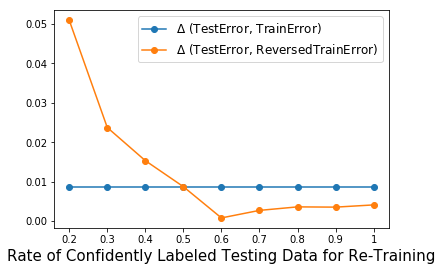
\includegraphics[width=5.5cm,height=3.5cm]{exp1_confidence.png}
\vspace{-10pt}
\caption{$\Delta_{tr}$ and $\Delta_{retr}$ versus Re-training Sample Size}
\label{exp1:confidence}
\end{figure}

{\noindent \bf Results on other data sets based on 
other models} 

Now we evaluate Algorithm \ref{alg:prediction} 
extensively on multiple data sets, based on different 
base models and prediction quality metrics. 
Let $\tilde{f1}(f; S)$ be the reversed f1-score. 
Results are shown in Table \ref{tab1:accf1}. 

We see $\tilde{er}(f; S)$ is a more 
accurate estimate of $er(f; Q)$ than $er(f; S)$, 
and $\tilde{f1}(f; S)$ is a more accurate 
estimate of $f1(f; Q)$ than $f1(f; S)$. 
These observations are consistent across different 
base models and different data sets. 
An exception is on the Malware data set. 
This may be because the testing error on this data set 
is very large (around 0.38), thus pseudo-labels are 
mostly wrong and significantly mislead $f$ in its retraining. 
This suggests reversed testing quality is more effective 
when prediction quality is relatively high. 






























